\documentclass[11pt, letterpaper]{memoir}
\usepackage{HomeworkStyle}
\geometry{margin=1in}



\begin{document}

	\begin{center}
		{\large Quiz 4.1 -- Chemical Potential and Phase Diagrams}
	\end{center}
	{\large Name: \rule[-1mm]{4in}{.1pt} 
		
\subsection*{Chemical Potential}
Chemical potential, $\mu$, is related to $G$ in a way that is sometimes hard to disentangle. What exactly is the relationship between $\mu$ and $G$?

\vspace{4em}
\subsection*{Phase Diagrams}

\hspace{-3em}
\begin{minipage}{0.4\linewidth}
	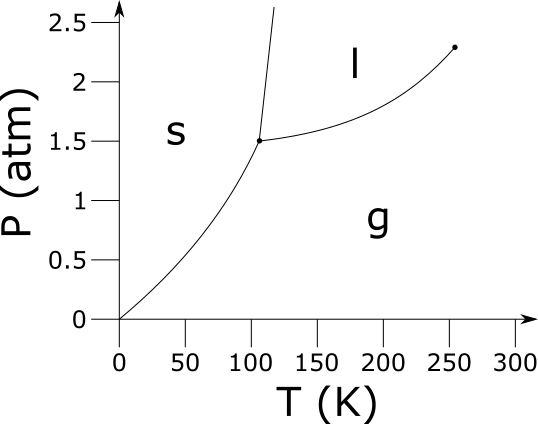
\includegraphics[width=\textwidth]{Phase_Diagram}
\end{minipage}
\begin{minipage}{0.7\linewidth}
	Use the phase diagram at left to answer the following questions:
	
	\noindent
	\begin{itemize}
		\item What is the stable phase at $2.25~atm$ and $200~K$?
		\item Give $T$ and $p$ for the triple point and the critical point
		
		\vspace{2em}
		\item Estimate the vapor pressure at $50~K$ and at $200~K$ 
		
		\vspace{2em}
		~
	\end{itemize}
\end{minipage}

\vspace{2em}\noindent\hspace{-2em}
\begin{minipage}{0.7\linewidth}
	Use the phase diagram at right to answer the following questions:
	
	\noindent 
	\begin{itemize}
		\item How many solid phases are represented?
		
		\item Highlight all parts of the diagram where there is only 1 free variable (i.e. variance = 1)	
		
		\item Indicate a forbidden point on the diagram		
			
		
		\item List the solid phases from least dense to most dense
		
		\vspace{2em}
		
		\item Which solid phase has the greatest molar entropy?
		
		\vspace{2em}
		\item A sample begins at $2.5~atm$ and $200~K$. What phase changes would occur as the pressure is isothermally reduced to $0~atm$?
	\end{itemize}
\end{minipage}~
\begin{minipage}{0.4\linewidth}
	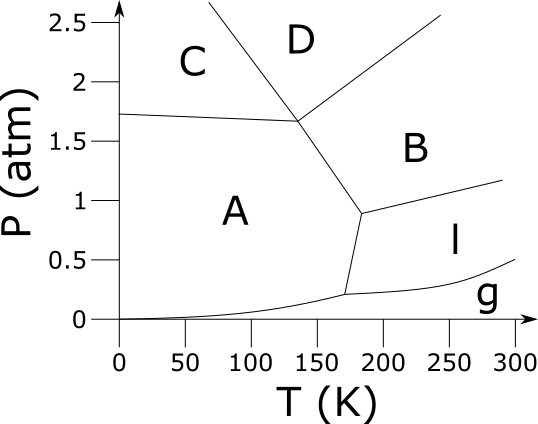
\includegraphics[width=\textwidth]{Phase_Diagram2}
\end{minipage}

\newpage
\pagestyle{empty}
\addtocounter{page}{-1}
\section*{\emph{{\fontspec{Microsoft JhengHei}游子吟} (Song of a Traveling Son)}}
\paragraph{By {\fontspec{Microsoft JhengHei}孟郊} (Meng Jiao)}~
{\fontspec{Microsoft JhengHei}
	\begin{verse}	
		慈 母 手 中 线, 游 子 身 上 衣 。\\
		临 行 密 密 缝, 意 恐 迟 迟 归 。\\
		谁 言 寸 草 心, 报 得 三 春 晖 。
	\end{verse}
}

\vspace{2em}
\begin{verse}
	Thread in the hands of a loving mother\\
	Turns to clothes on the traveling son.\\
	She adds stitch after tight stitch until he leaves\\
	and worries about his return.\\
	A grass blade is bathed in spring sun;\\
	how can its inch-sized heart return such love?
\end{verse}
\end{document}
